\section{Estudio de la respuesta de los sensores del robot humanoide TEO y la aplicación de su información al control del equilibrio}

En este capítulo se van a exponer las respuestas de los sistemas sensoriales del robot humanoide TEO a diferentes inclinaciones  para simular perturbaciones pequeñas que cambian la posición del ZMP y mantener el equilibrio del robot haciendo uso de la estrategia de control de los tobillos. Para ello se decidió ajustar un modelo (el modelo de péndulo invertido lineal) de los dos actuales existentes y a partir de él ajustar el otro (el modelo cart-table).

\subsection{Estudio de la respuesta de los sensores F-T}

Para estudiar la respuesta de los sensores F-T ante perturbaciones y aplicar dicha información obtenida al modelo LIPM, y poder así desarrollar un nuevo modelo personalizado, se ha seguido una serie de pasos divididos en tres fases: fase experimental, fase de análisis de datos y fase de validación de resultados, que se ilustran en la figura \ref{figura51}. 

\begin{figure}[H]
\centering
\includegraphics[scale=0.5]{imagenes/apartado_5/51_diagrama_desarrollo_nuevo_modelo}
\caption{Diagrama del desarrollo experimental del nuevo modelo}
\label{figura51}
\end{figure}

\begin{comment}
Como se ha comentado en el capítulo 4, existen errores provenientes de la información de los sensores F-T de los tobillos del robot debido a los efectos que aparecen en los pares y fuerzas medidos por los sensores cuando éste es sometido a una perturbación de su equilibrio, por lo que se hace necesario separar las inexactitudes de las mediciones y la información relacionada con el comportamiento esperado ante dichas perturbaciones.

Para ello es necesario primero establecer las variables que intervienen en el proceso (CoM y masa) y segundo, definir una estrategia para su control. 

A partir de los experimentos desarrollados se ha podido establecer un método para desarrollar el nuevo modelo. Se recogen y procesan los datos obtenidos de los sensores F-T de los experimentos del sistema en bucle abierto. Con esta información, se calcula el $X_{ZMP_{F-T}}$ real y se compara con el $X_{ZMP_{exp}}$ esperado. De aquí se puede observar que hay una diferencia, el error anteriormente comentado, por lo que para corregirlo éste se modela, obteniendo una ecuación para describir dicho error. Una vez obtenido el error modelado, éste se incluye en el modelo original como una fuerza ficticia que corrige la diferencia, obteniéndose el nuevo modelo utilizado a lo largo del actual proyecto. A partir del mismo se puede observar como el comportamiento del ZMP medido y el planificado son similares. Dicho proceso se puede observar en los siguientes apartados.
\end{comment}

\subsubsection{Descripción de la metodología experimental}

Los experimentos han seguido una serie de pasos para que las lecturas fueran correctas. Éstos se dividen en:

NOTA: Los primeros 2 pasos deben realizarse con el robot en suspensión, es decir, sin que toque el suelo con la suela de los pies. A continuación se explicará el motivo.

\begin{enumerate}

%%\item \textbf{Encendido del robot}\\ Encender la fuente de alimentación del robot y el robot junto a sus CPU's, tanto Manipulation como Locomotion.

%%\item \textbf{Iniciar CPU's en el ordenador}\\ Desde el ordenador, deberemos iniciar las CPU's de Manipulation primero y la de Locomotion después, ya que dentro de manipulation se encuentra el YarpServer necesario para la conexión de todos los elementos del robot con el ordenador.

\item \textbf{Puesta del robot en posición inicial (Homeposs)}\\ Una vez se ha encendido el robot y las CPU's se va a proceder a la puesta a cero de la posición del mismo, ya que puede haber modificaciones en su posición de anteriores experimentos o simplemente para asegurarse que los experimentos salen correctamente y siempre empiezan desde la misma posición de inicio. Esto debe realizarse con el robot en suspensión para evitar posibles colisiones de los pies con el suelo.

\item \textbf{Corrección offset sensores F-T}\\ Siguiendo con el robot en suspensión y una vez realizada la posición de inicio, desde una terminal se deben iniciar los sensores F-T de los tobillos que se van a encargar de dar la información de las fuerzas y los pares al programa para así poder realizar los experimentos y eliminar los posibles offset que puedan tener los mismos. Es importante que no esté apoyado en el suelo para que cuando se ejecute esta corrección, no se elimine el valor de la fuerza ejercida por la masa del robot. Una vez que se han iniciado los sensores F-T de los tobillos ya se podría bajar el robot para que éstos puedan tener en cuenta su propio peso y las demás fuerzas y pares. 
%%empiecen a tener el cuenta el peso del propio robot mediante la fuerza de reacción que se genera entre el mismo y el suelo, ya que con él en suspensión los sensores miden pero esas lecturas son de la gravedad.

\item \textbf{Puesta en funcionamiento del programa}\\ Cuando se inicia el programa, existe una primera fase en la que el robot no realiza ningún movimiento. Esto se debe a que se está configurando de tal manera que se elimine el offset que pueda haber al inicio debido a la posición de homeposs del robot, ya que ésta no es perfecta y, debido a la flexibilidad de la estructura y otros errores acumulados, puede no estar totalmente erguido y que las fuerzas en el plano axial no sean cero. 

Una vez que ha pasado esta fase, y estamos seguros de que ese offset se ha eliminado en la medida de lo posible, se envía al robot un $ZMP_{ref}$ \footnote{ZMP de referencia al que el robot debería llegar atendiendo a la física y cálculos teóricos del modelo LIPM} y TEO comanda un ángulo, que ha calculado a partir de la conversión del $ZMP_{ref}$, activando los motores de sus tobillos (inclinando el robot dicho ángulo) y calculando el $ZMP_{F-T}$ del modelo de péndulo invertido lineal hasta que este $ZMP_{F-T}$ se estabiliza, para hacer coincidir tanto la parte transitoria como la parte de régimen permanente del $ZMP_{F-T}$ con el del $ZMP_{ref}$.

\end{enumerate}

\begin{figure}[H]
\centering
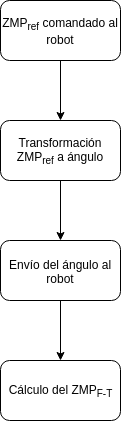
\includegraphics[scale=0.5]{imagenes/apartado_5/52_diagrama_flujo1}
\caption{Diagrama de flujo del programa}
\label{figura52}
\end{figure}


\subsubsection{Respuesta del sistema LIPM}

Para poder establecer el nuevo modelo lo primero que hay que hacer es fijar las variables que intervienen en el modelo. La masa del robot TEO es de 62,6 kg y la altura desde el suelo al CoM es 0,893 m (la longitud del péndulo). El siguiente paso que se realizó fue someter al robot a una serie de variaciones en el ángulo de los tobillos para simular perturbaciones pequeñas, con la excepción de que no volvía al ZMP inicial, para así poder modelar mejor la diferencia entre el ZMP esperado y el medido, estudiándose también su variación dinámica a lo largo del proceso. 

En el presente proyecto se ha llevado a cabo una batería de 30 experimentos. El plano sagital (x-z) en el que se desarrollaron está representado en la figura \ref{figura53}. Esta metodología también se podría aplicar para cualquier otro plano espacial ya que se obtuvieron resultados similares en el plano frontal (y-z).

\begin{figure}[H]
\centering
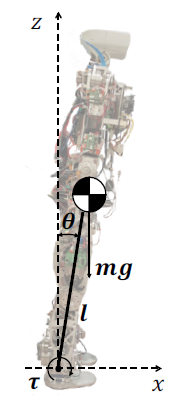
\includegraphics[scale=0.65]{imagenes/apartado_5/53_postura_inicial_experimental_teo}
\caption{Plano de desarrollo de los experimentos del robot TEO}
\label{figura53}
\end{figure}

La metodología utilizada en los primeros experimentos seguía el siguiente esquema:

\begin{figure}[H]
\centering
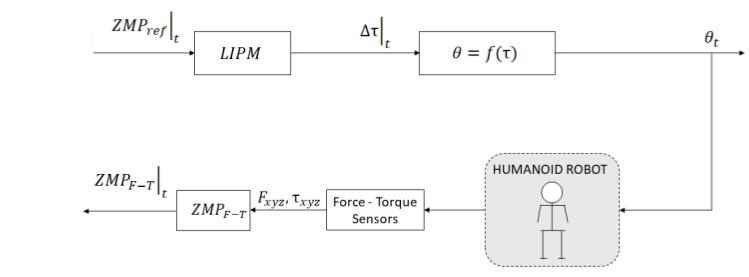
\includegraphics[scale=2.2]{imagenes/apartado_5/54_esquema_bucle_abierto}
\caption{Control de posición básico del ZMP usando el modelo LIPM}
\label{figura54}
\end{figure}


En ellos se ajustó la altura del CoM del modelo LIPM para reducir lo máximo posible la diferencia entre el ZMP calculado de los F-T y el ZMP deseado. Esta evolución se puede observar de la figura \ref{figura55}, en la que se mejoró la respuesta del sistema pero en la que todavía se mostraba un error en régimen permanente. Como se puede observar, a mayor ZMP el ángulo de inclinación es mayor y el robot es más inestable debido a que éste se encuentra más cerca del borde del polígono de soporte, y los errores tienen mayor influencia, principalmente los que tienen que ver con la flexibilidad de la estructura del robot y sus tolerancias mecánicas. Estos errores se pueden ver en el régimen permanente de la figura \ref{figura55} b). También se observa una oscilación inicial muy grande, algo que se tiene que evitar sobre todo cuando el ZMP se encuentra en el borde del polígono de apoyo. 

\begin{figure}[H]
\centering
\subfigure{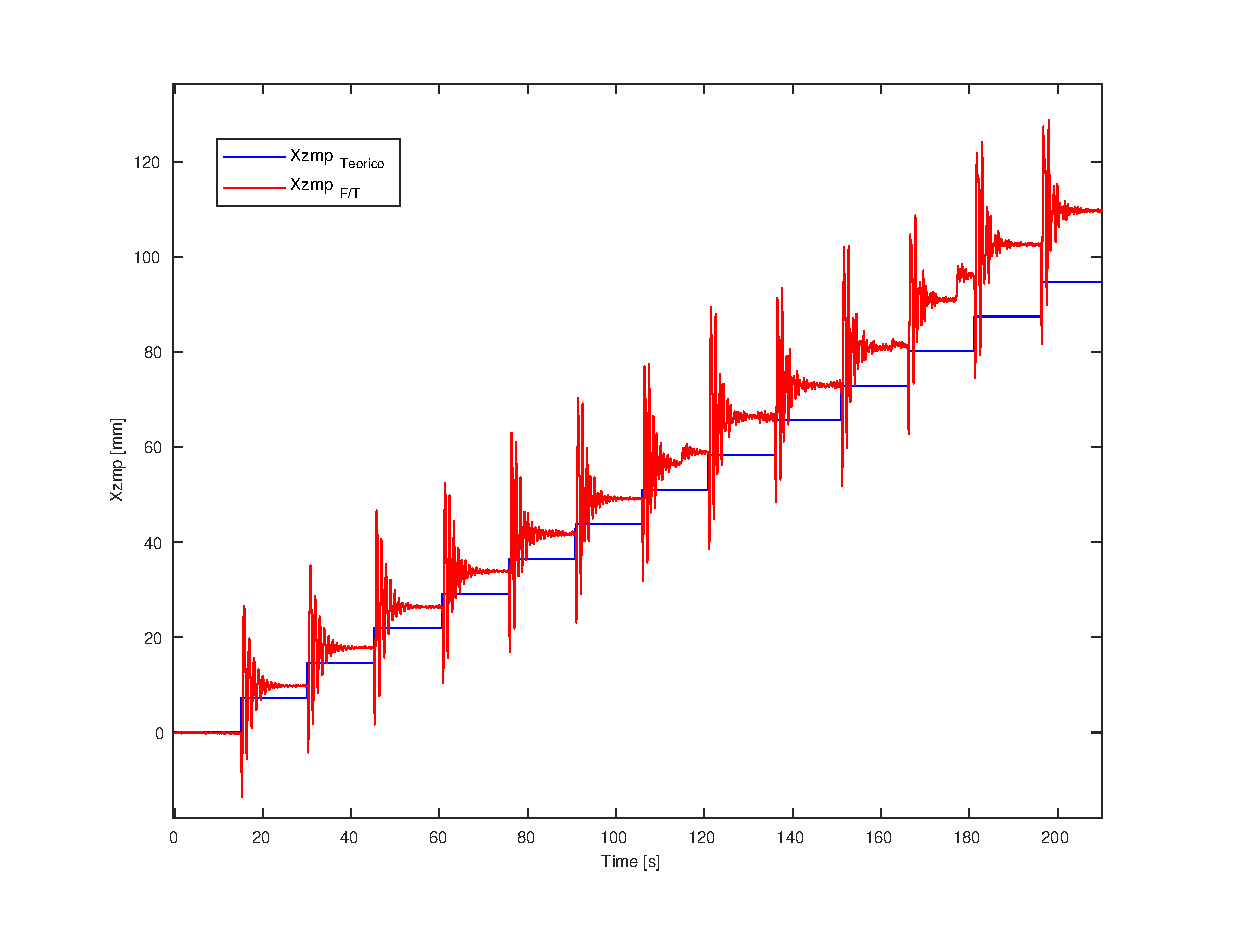
\includegraphics[scale=0.2]{imagenes/apartado_5/55_1_altura_no_ajustada}}
\quad
\subfigure{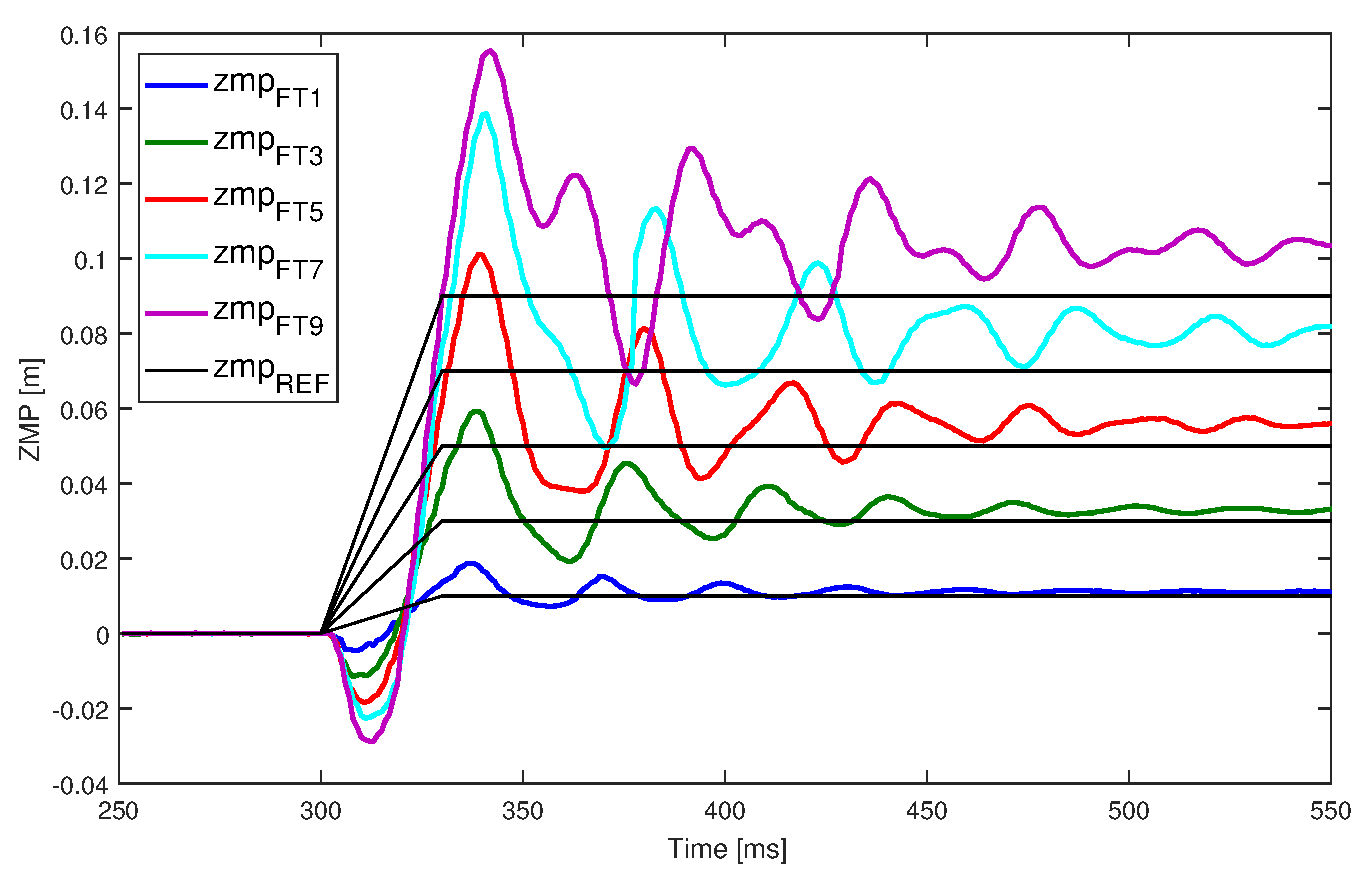
\includegraphics[scale=0.2]{imagenes/apartado_5/55_2_altura_ajustada.pdf}}
\caption{Evolucion ZMP modelo LIPM}
\label{figura55}
\end{figure}

\begin{comment}
\begin{figure}[H]
\centering
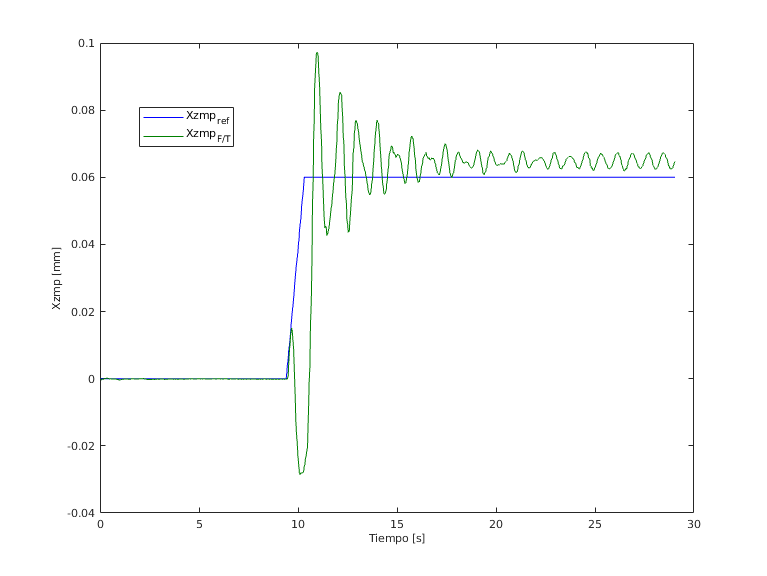
\includegraphics[width=13cm, height=8cm]{imagenes/apartado_5/5.1/54_evolucion_zmpref_5mm}
\caption{Evolución ZMP modelo LIPM para ZMPref = 5mm}
\label{figura54}
\end{figure}
\end{comment}



%aquí introducir la imagen con la evolución de los experimentos



%%NOTA: En el gráfico de la figura \ref{figura54} se puede observar que a pesar de realizar un control/corrección sobre el ángulo que se comanda al robot a partir de la conversión del $ZMP_{ref}$, el $ZMP_{F-T}$ nunca llega a estabilizarse y esto es debido a que continuamente se está corrigiendo el ángulo de inclinación.

En los siguientes experimentos, representados en la tabla \ref{tabla51}, se programó un controlador en ZMP para mejorar la respuesta del sistema y reducir el error tanto en régimen permanente como en el transitorio. Se fueron ajustando las variables de dicho controlador para comprobar si el $ZMP_{F-T}$ se podía estabilizar. La arquitectura de control de los experimentos se muestra en la figura \ref{figura56}.

\begin{figure}[H]
\centering
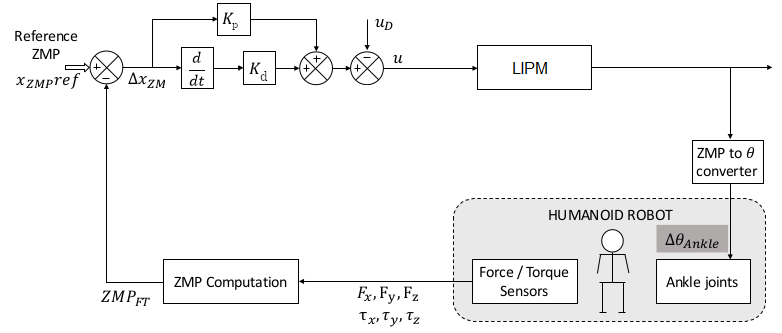
\includegraphics[scale=0.6]{imagenes/apartado_5/56_esquema_bucle_cerrado}
\caption{Arquitectura de control de ZMP mediante controlador PD}
\label{figura56}
\end{figure}


\begin{table}[H]
\begin{center}
\begin{tabular}{|c|c|c|c|}
\hline
Exp. & $k_p$   & $k_d$    & $k_u$ \\ \hline
1    & -0.0025 & 0.00005  & 1    \\ \hline
2    & -0.0025 & 0.00005  & 1.2  \\ \hline
3    & -0.0025 & 0.00005  & 1.4  \\ \hline
4    & -0.0025 & 0.00005  & 2    \\ \hline
5    & -0.005  & 0.0005   & 1    \\ \hline
6    & -0.005  & 0.0005   & 1.65 \\ \hline
7    & -0.01   & 0.0005   & 1    \\ \hline
8    & -0.01   & 0.0005   & 1.65 \\ \hline
9    & -0.05   & 0.005    & 1.65 \\ \hline
10   & -0.015  & -0.00025 & 1.4  \\ \hline
11   & -0.035  & -0.0001  & 1.4  \\ \hline
\end{tabular}
\end{center}
\caption{Batería de experimentos}
\label{tabla51}
\end{table}

\begin{figure}[H]
\centering
\subfigure[Experimento 1]
{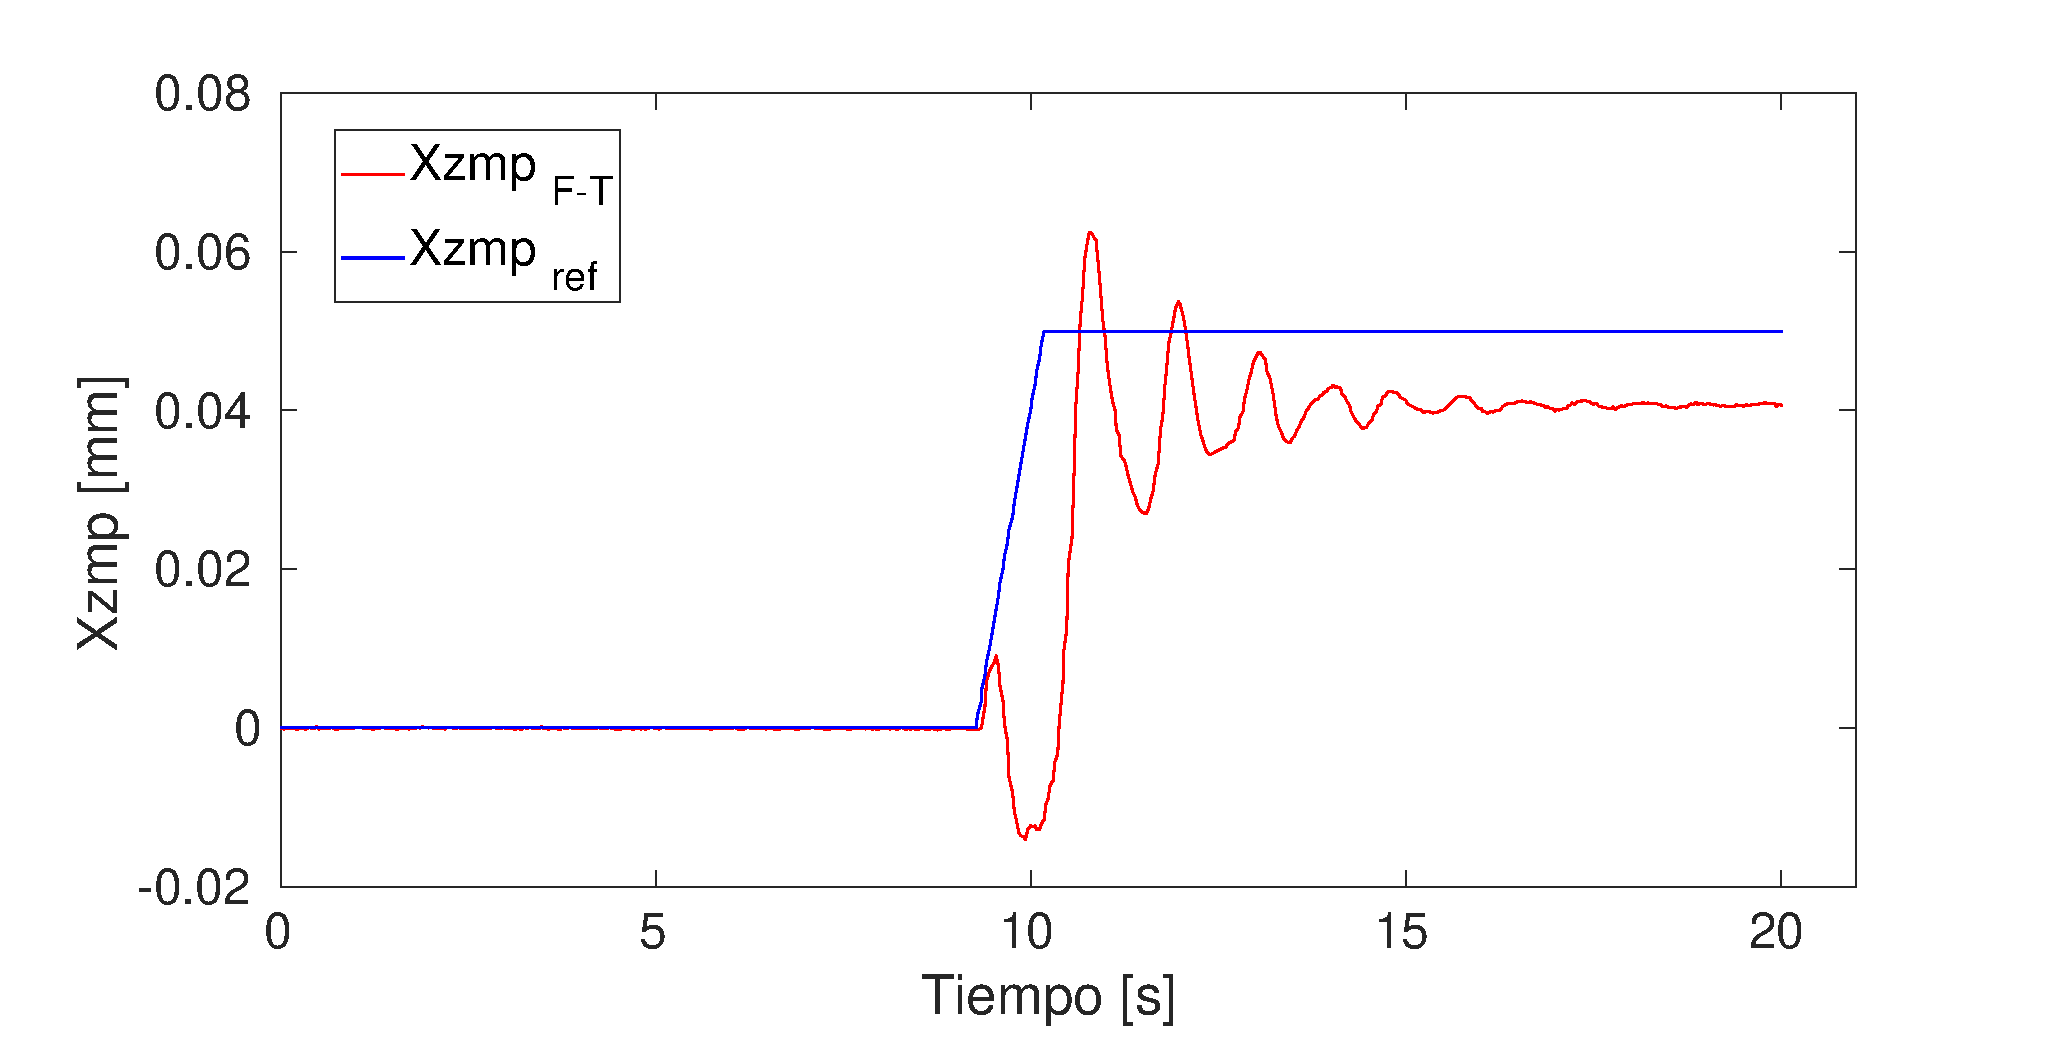
\includegraphics[scale=0.2]{imagenes/apartado_5/57_1_exp1}}
\quad
\subfigure[Experimento 3]
{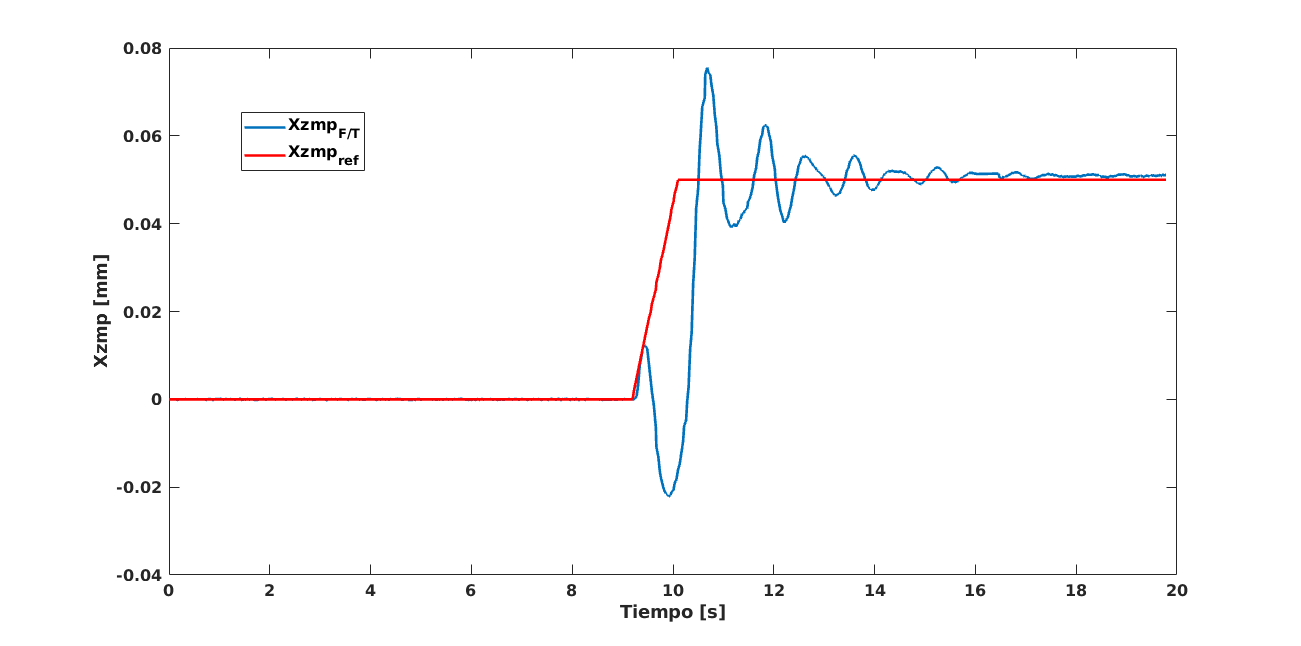
\includegraphics[scale=0.2]{imagenes/apartado_5/57_2_exp3}}
\quad
\subfigure[Experimento 5]
{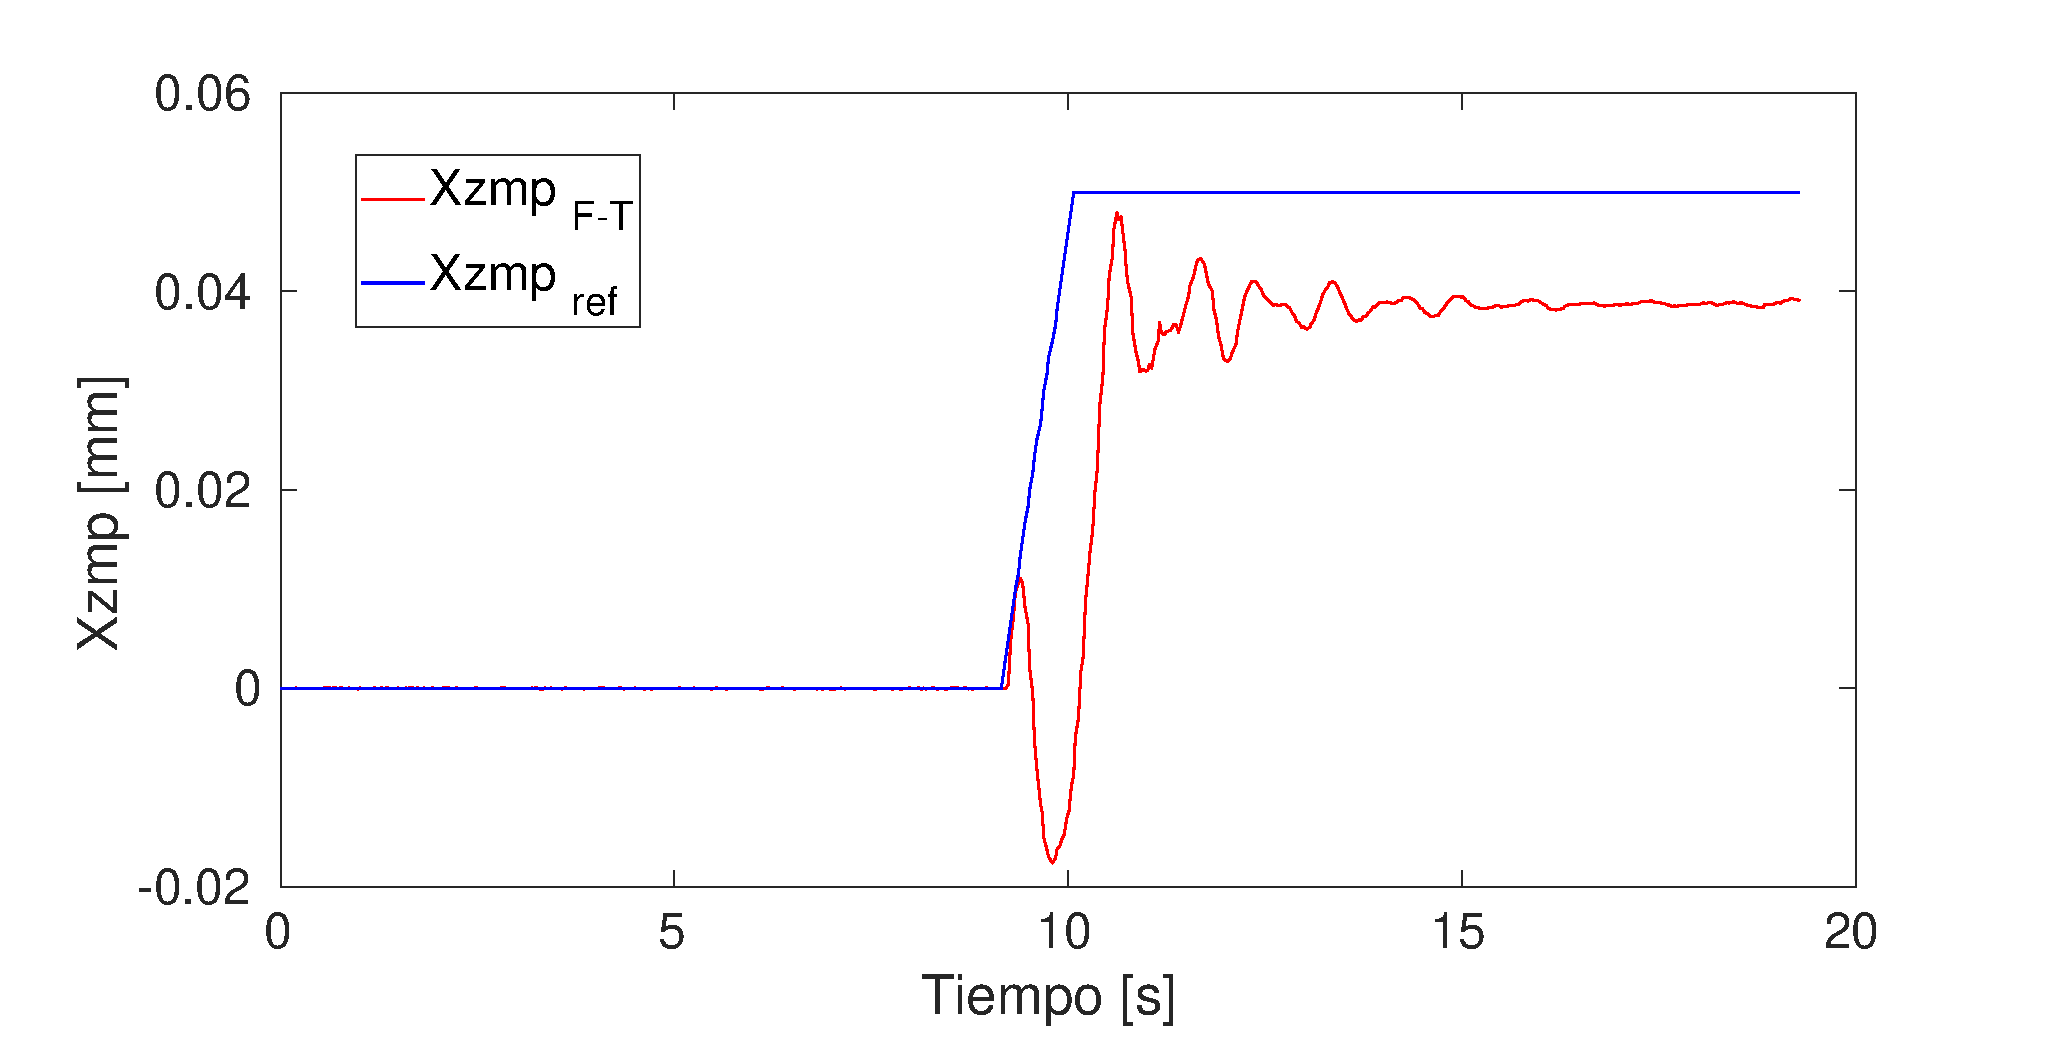
\includegraphics[scale=0.2]{imagenes/apartado_5/57_3_exp5}}
\quad
\subfigure[Experimento 10]
{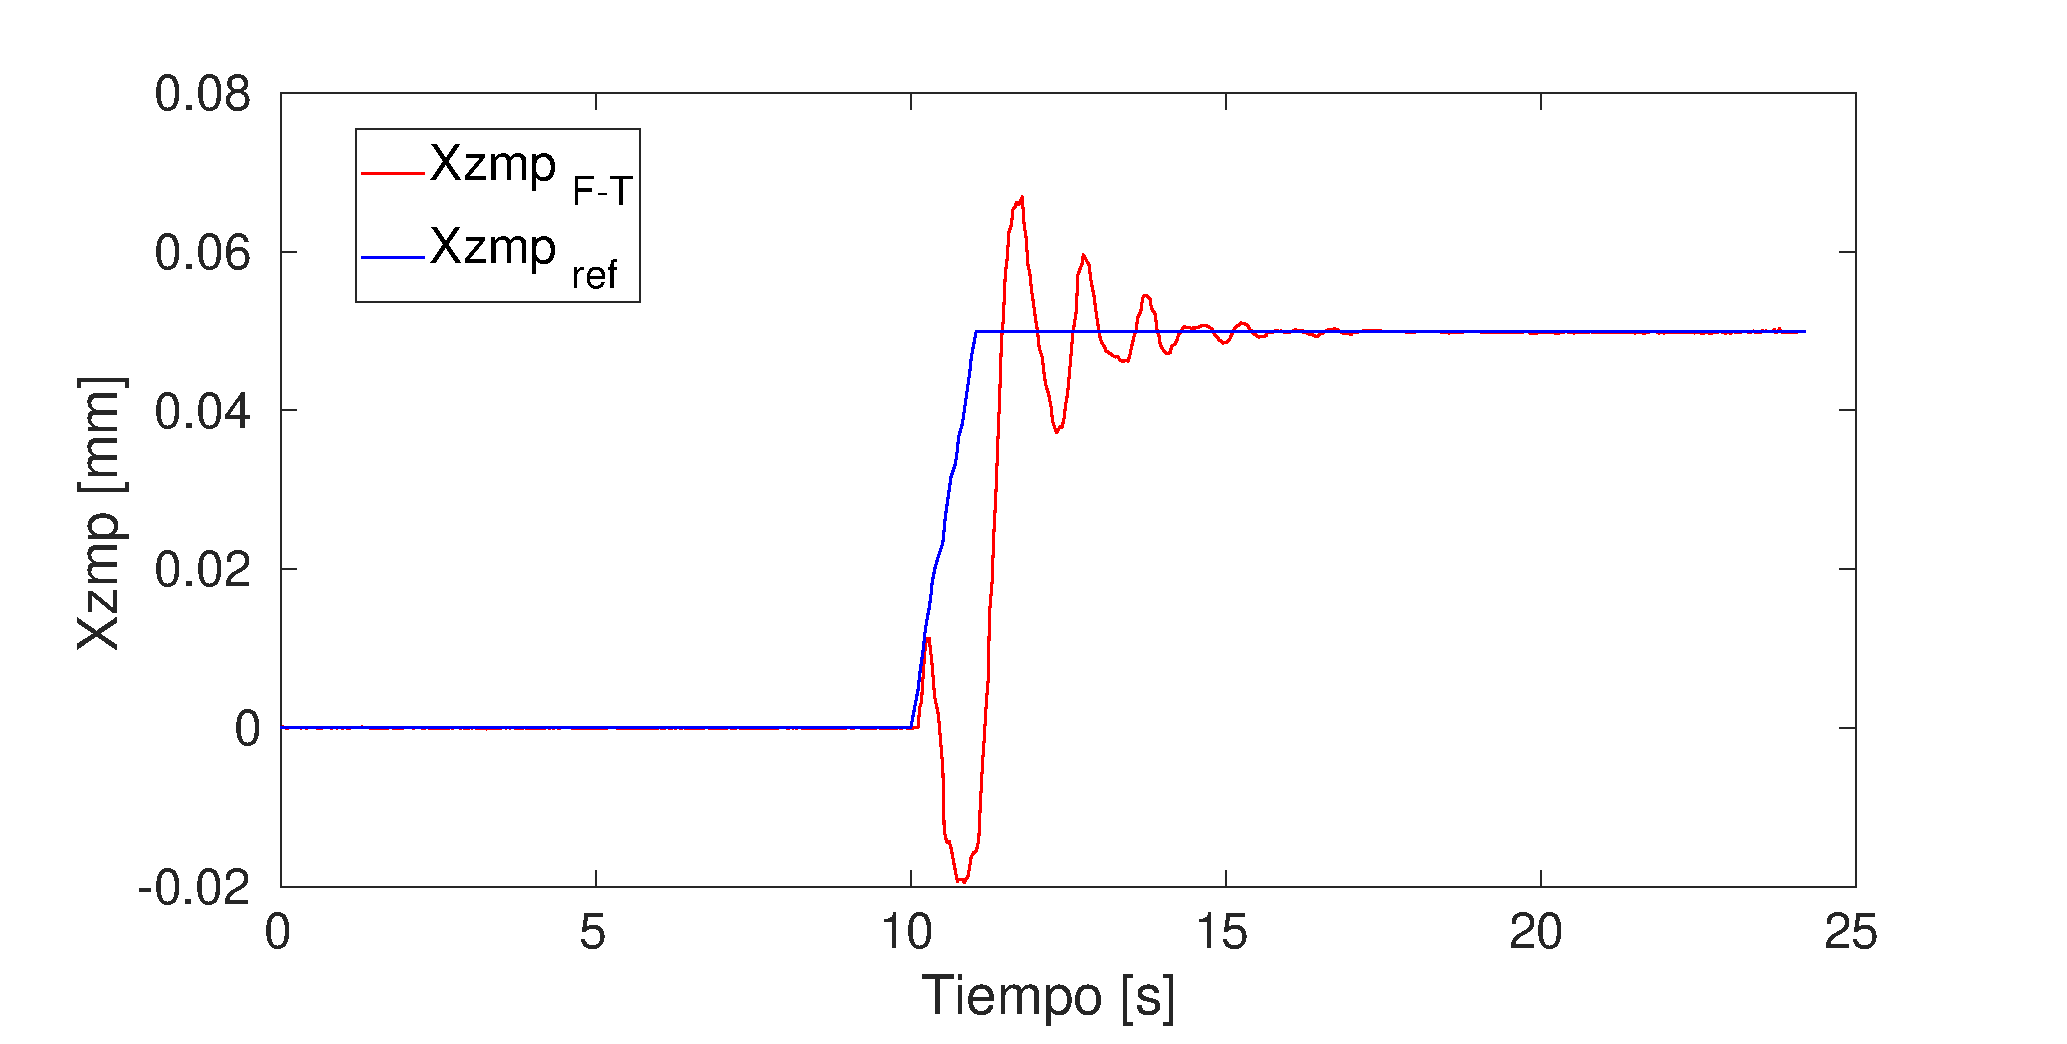
\includegraphics[scale=0.2]{imagenes/apartado_5/57_4_exp10}}
\quad
\subfigure[Experimento 11]
{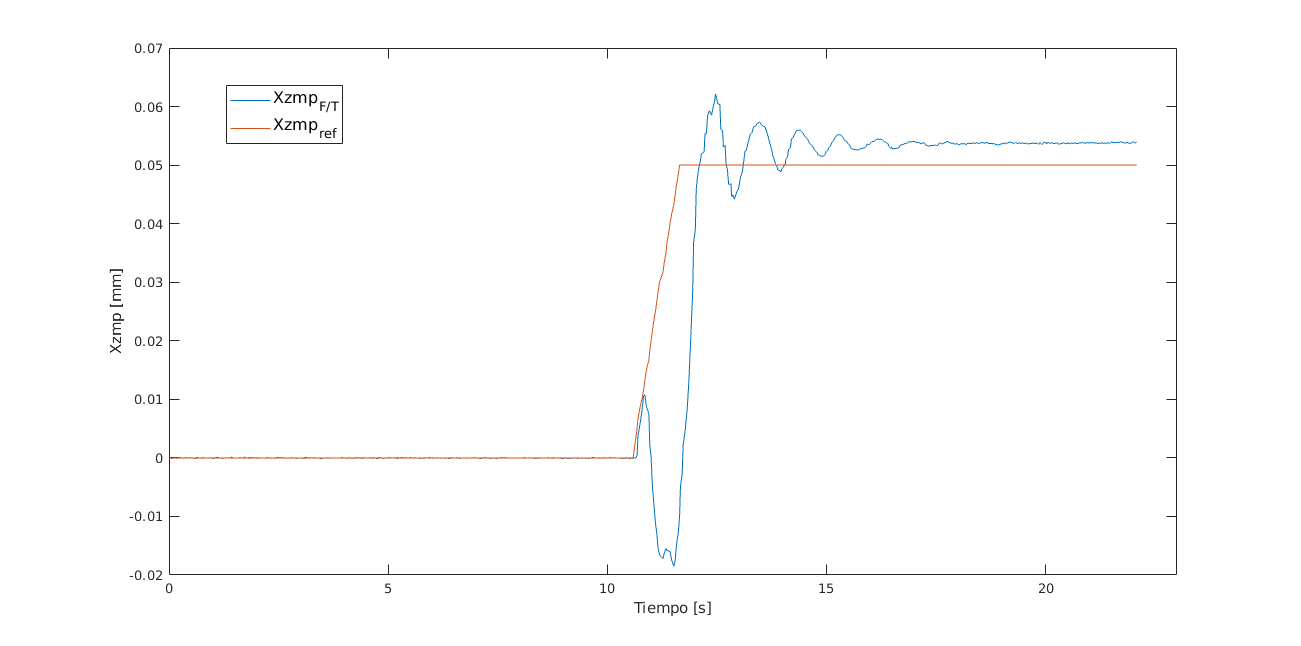
\includegraphics[scale=0.2]{imagenes/apartado_5/57_5_exp11}}
\caption{Evolución ZMP para ZMPref = 5mm}
\label{figura57}
\end{figure}

%% el comment siguiente son las figuras justo encima de este comentario, pero situadas individualmente

\begin{comment}
\begin{figure}[H]
\centering
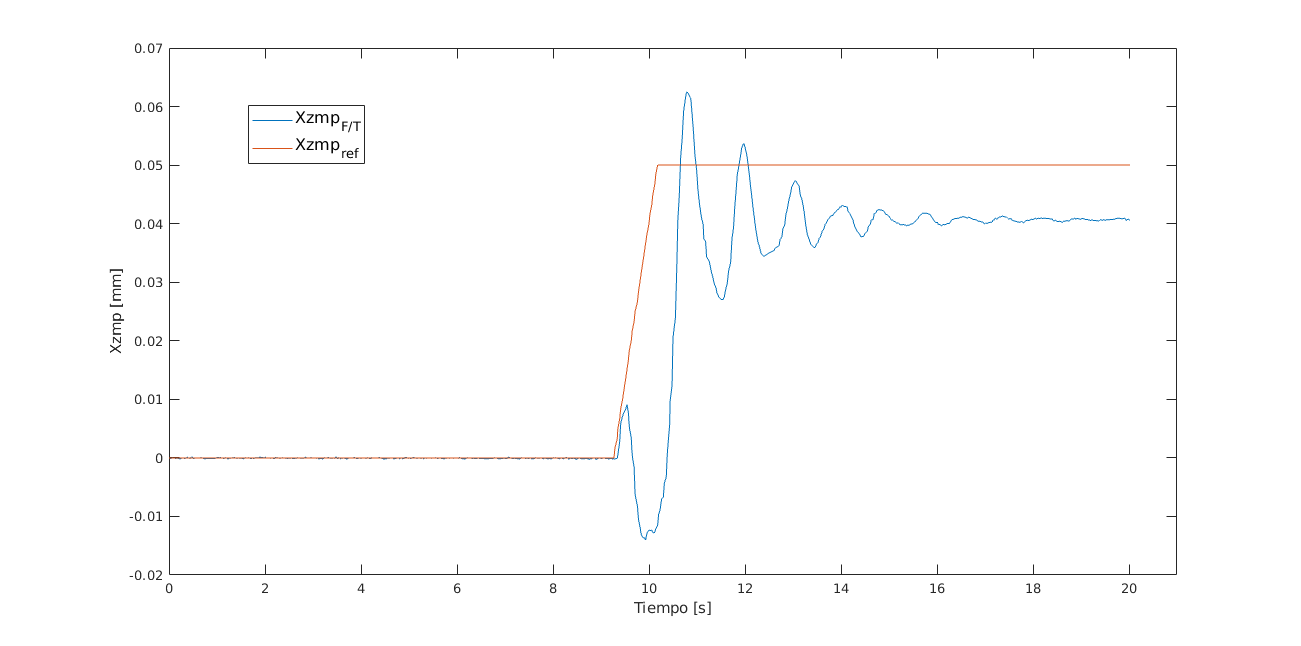
\includegraphics[width=13cm, height=8cm]{imagenes/apartado_5/5.1/55}
\caption{Evolución ZMP experimento 1 para ZMPref = 5mm}
\label{figura55}
\end{figure}

\begin{figure}[H]
\centering
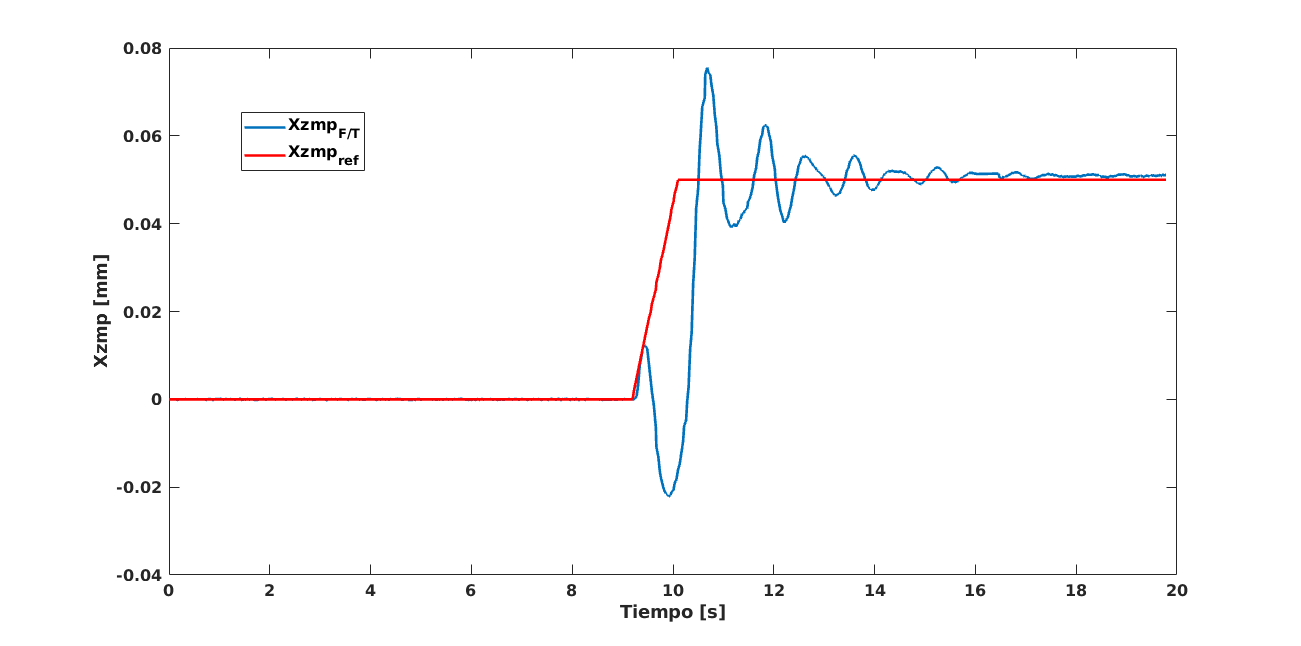
\includegraphics[width=13cm, height=8cm]{imagenes/apartado_5/5.1/56}
\caption{Evolución ZMP experimento 3 para ZMPref = 5mm }
\label{figura56}
\end{figure}

\begin{figure}[H]
\centering
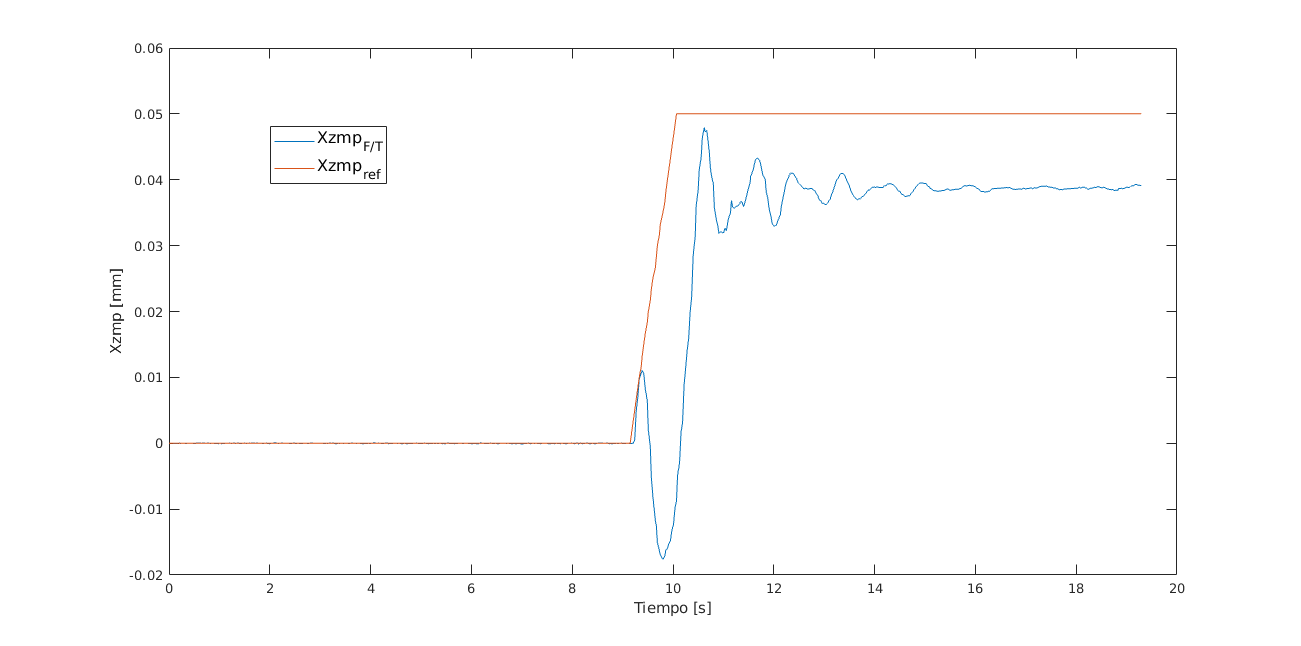
\includegraphics[width=13cm, height=8cm]{imagenes/apartado_5/5.1/57}
\caption{Evolución ZMP experimento 5 para ZMPref = 5mm}
\label{figura57}
\end{figure}

\begin{figure}[H]
\centering
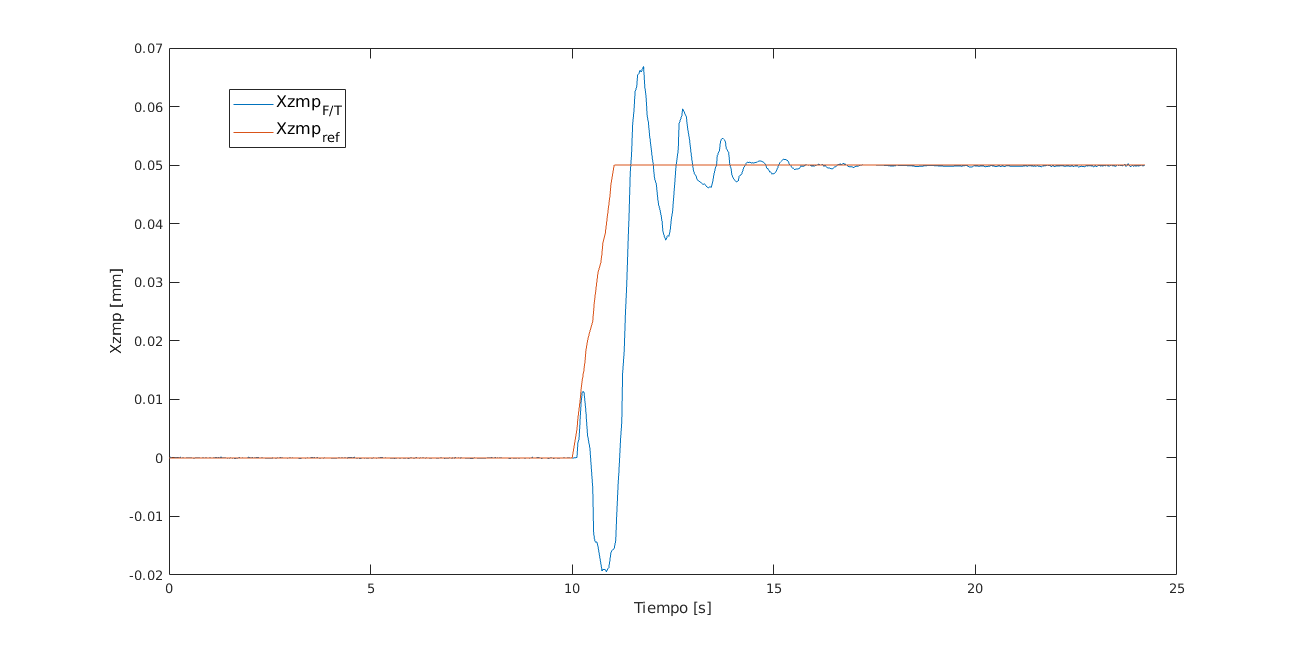
\includegraphics[width=13cm, height=8cm]{imagenes/apartado_5/5.1/58}
\caption{Evolución ZMP experimento 10 para ZMPref = 5mm}
\label{figura58}
\end{figure}

\begin{figure}[H]
\centering
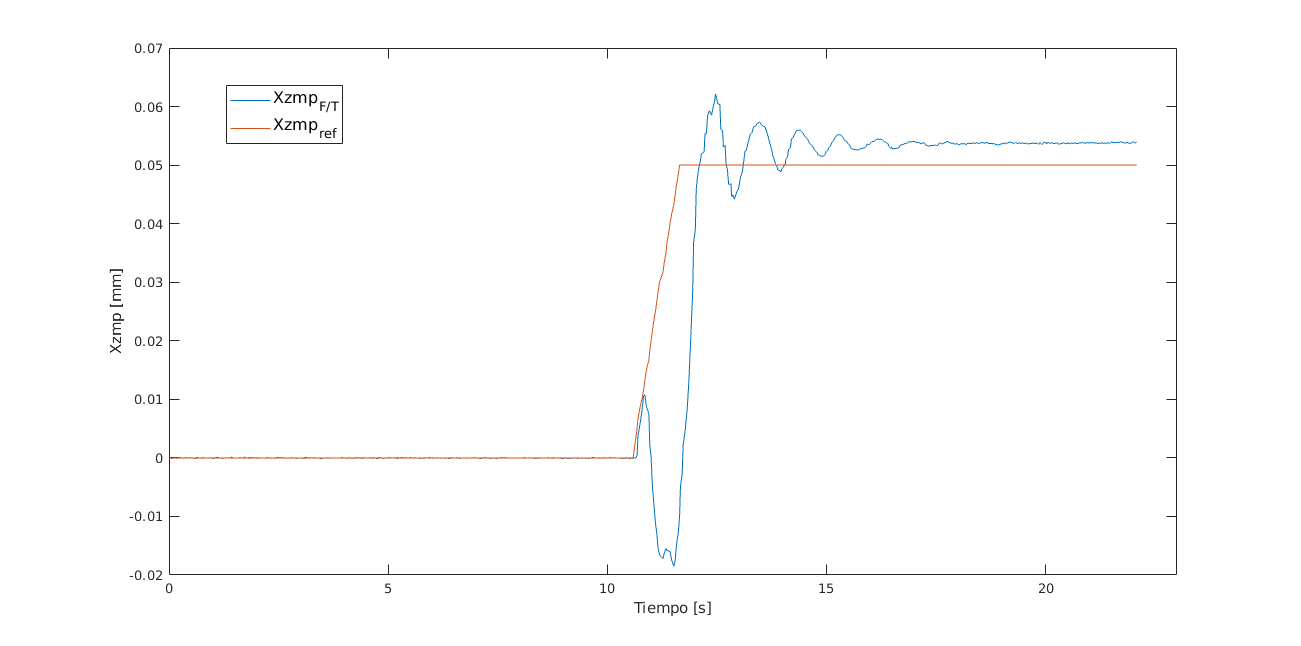
\includegraphics[width=13cm, height=8cm]{imagenes/apartado_5/5.1/59}
\caption{Evolución ZMP experimento 11 para ZMPref = 5mm}
\label{figura59}
\end{figure}
\end{comment}

%aquí introducir las gráficas de zmp_ft y zmp_ref frente al ángulo en grados (deg) 

En las pruebas representadas en la figura \ref{figura57}, cuando se lograba ajustar la respuesta en régimen permanente, reduciendo el error entre el $ZMP_{F-T}$ y el ZMP deseado, el régimen transitorio tenía una oscilación muy grande, y como se ha comentado antes esto se tiene que evitar sobre todo en ZMP situados en el borde del polígono de soporte. Por el contrario si se lograba hacer la oscilación inicial un poco más pequeña el tiempo de estabilización del sistema era mayor, por lo que éste se volvía más lento y no se lograba reducir el error del régimen permanente. Es por ello que se hace necesario la mejora del modelo LIPM, tanto para eliminar el error de régimen permanente como para reducir la oscilación y el sobrepaso del régimen transitorio.

\subsubsection{Modelado de la respuesta del ZMP}

\begin{itemize}

\item \textbf{Modelo de Péndulo Lineal Invertido Dinámico}

Como se ha explicado en el apartado \ref{definicionDLIPM}, se ha aplicado una mejora al modelo LIPM que permitía mejorar de manera dinámica la respuesta del sistema.

Aplicando Laplace a la ecuación de la física del movimiento del nuevo modelo, la función de transferencia quedaría:

\begin{comment}
\begin{equation}
\begin{split}
-ml{\theta}(S)S^{2} - B_a l{\theta}(S)S - k_a l\theta(S) + mg\theta(S)=- X(S) \cdot mg\\
{\theta}(S)[-ml^{2}S^{2} - B_a lS + (-k_a l + mg)]=- X(S) \cdot mg \\
\frac{{\theta}(S)}{X(S)}=\frac{-mg}{-ml^{2}S^{2} - S B_a l + (-k_a l + mg)} \\
\frac{{\theta}(S)}{X(S)}=\frac{\frac{-g}{l^{2}}}{S^{2} - S (\frac{B_a}{ml}) + (\frac{k_a}{ml} - \frac{g}{l})}
\end{split}
\label{ec51}
\end{equation}
\end{comment}

\begin{equation*}
-ml{\theta}(S)S^{2} - B_a l{\theta}(S)S - k_a l\theta(S) + mg\theta(S)=- X(S) \cdot mg
\end{equation*}

\begin{equation*}
{\theta}(S)[-ml^{2}S^{2} - B_a lS + (-k_a l + mg)]=- X(S) \cdot mg
\end{equation*}

\begin{equation*}
\frac{{\theta}(S)}{X(S)}=\frac{-mg}{-ml^{2}S^{2} - S B_a l + (-k_a l + mg)}
\end{equation*}

\begin{equation}
\frac{{\theta}(S)}{X(S)}=\frac{\frac{-g}{l^{2}}}{S^{2} - S (\frac{B_a}{ml}) + (\frac{k_a}{ml} - \frac{g}{l})}
\end{equation}

donde $\gamma=g/l^{2}$, $\alpha=B_{a}/ml$ y $\beta=(k_{a}/ml) - (g/l)$, quedaría simpificada:

\begin{equation}
\frac{\theta(S)}{X(S)}=\frac{\gamma}{S^{2}+\alpha S+\beta }
\label{ec52}
\end{equation}

. En el estado estable, cuando el tiempo pasa al infinito, la ganancia %%DC 
, que se encarga de eliminar el error del régimen permanente del sistema, sólo depende del parámetro $k_a$, como se indica en la ecuación \ref{ec53}.

\begin{equation}
K_{DC}=\frac{\gamma}{\beta}=\frac{k_{a} - g}{l}
\label{ec53}
\end{equation}

\item \textbf{Caracterización del error en régimen permanente}

El error anteriormente comentado entre el valor deseado de ZMP y el medido, que se detecta en la figura \ref{figura55}b), debe ser caracterizado. Es por ello que en la figura %%aqui poner la figura 16 del paper
se representa dicha desviación a partir de los datos de la figura \ref{figura551} y se realiza su estudio en cada punto experimental ($ZMP_{F-T}$). A partir de dicho estudio se saca una ecuación polinómica de segundo orden para modelar su desviación con respecto al $ZMP_{ref}$:

\begin{equation}
X_{ZMP_{F-T}} = a \cdot X_{ZMP_{ref}} + b \cdot X_{ZMP_{ref}} + c
\label{ec51}
\end{equation}

donde $a=0.834$, $b=1.024$ y $c=-0.0004$.

Una vez que el error estático se ha reducido, se debe mejorar la respuesta del régimen transitorio para reducir tanto el tiempo de estabilización como el nivel de las oscilaciones iniciales.

\item \textbf{Caracterización de la respuesta transitoria del ZMP}

Se ha demostrado que el la respuesta del robot humanoide como un péndulo invertido simple es un sistema subamortiguado. En dicho sistema se puede reducir las oscilaciones y modificar su respuesta global seleccionando adecuadamente tanto la ganancia como los parámetros dinámicos. En la figura \ref{figura58}, que muestra la diferencia entre las respuestas de las funciones de transferencia de los modelos LIPM y DLIPM ante una perturbación, se puede visualizar como dichos parámetros dinámicos pueden coger valores más altos en el modelo DLIPM, ya que posee un mayor margen de ajuste. Por ejemplo, en la ecuación \ref{ec428}, los parámetros dinámicos, que pueden obtenerse a partir de $\alpha$ que está relacionado con $B_a$, se pueden configurar de tal manera que se reduzca la sobreoscilación.

%%aquí va la figura 17 del paper, que es la figura 58 del tfg. Borrar este comentario cuando la incluya
\begin{figure}[H]
\centering
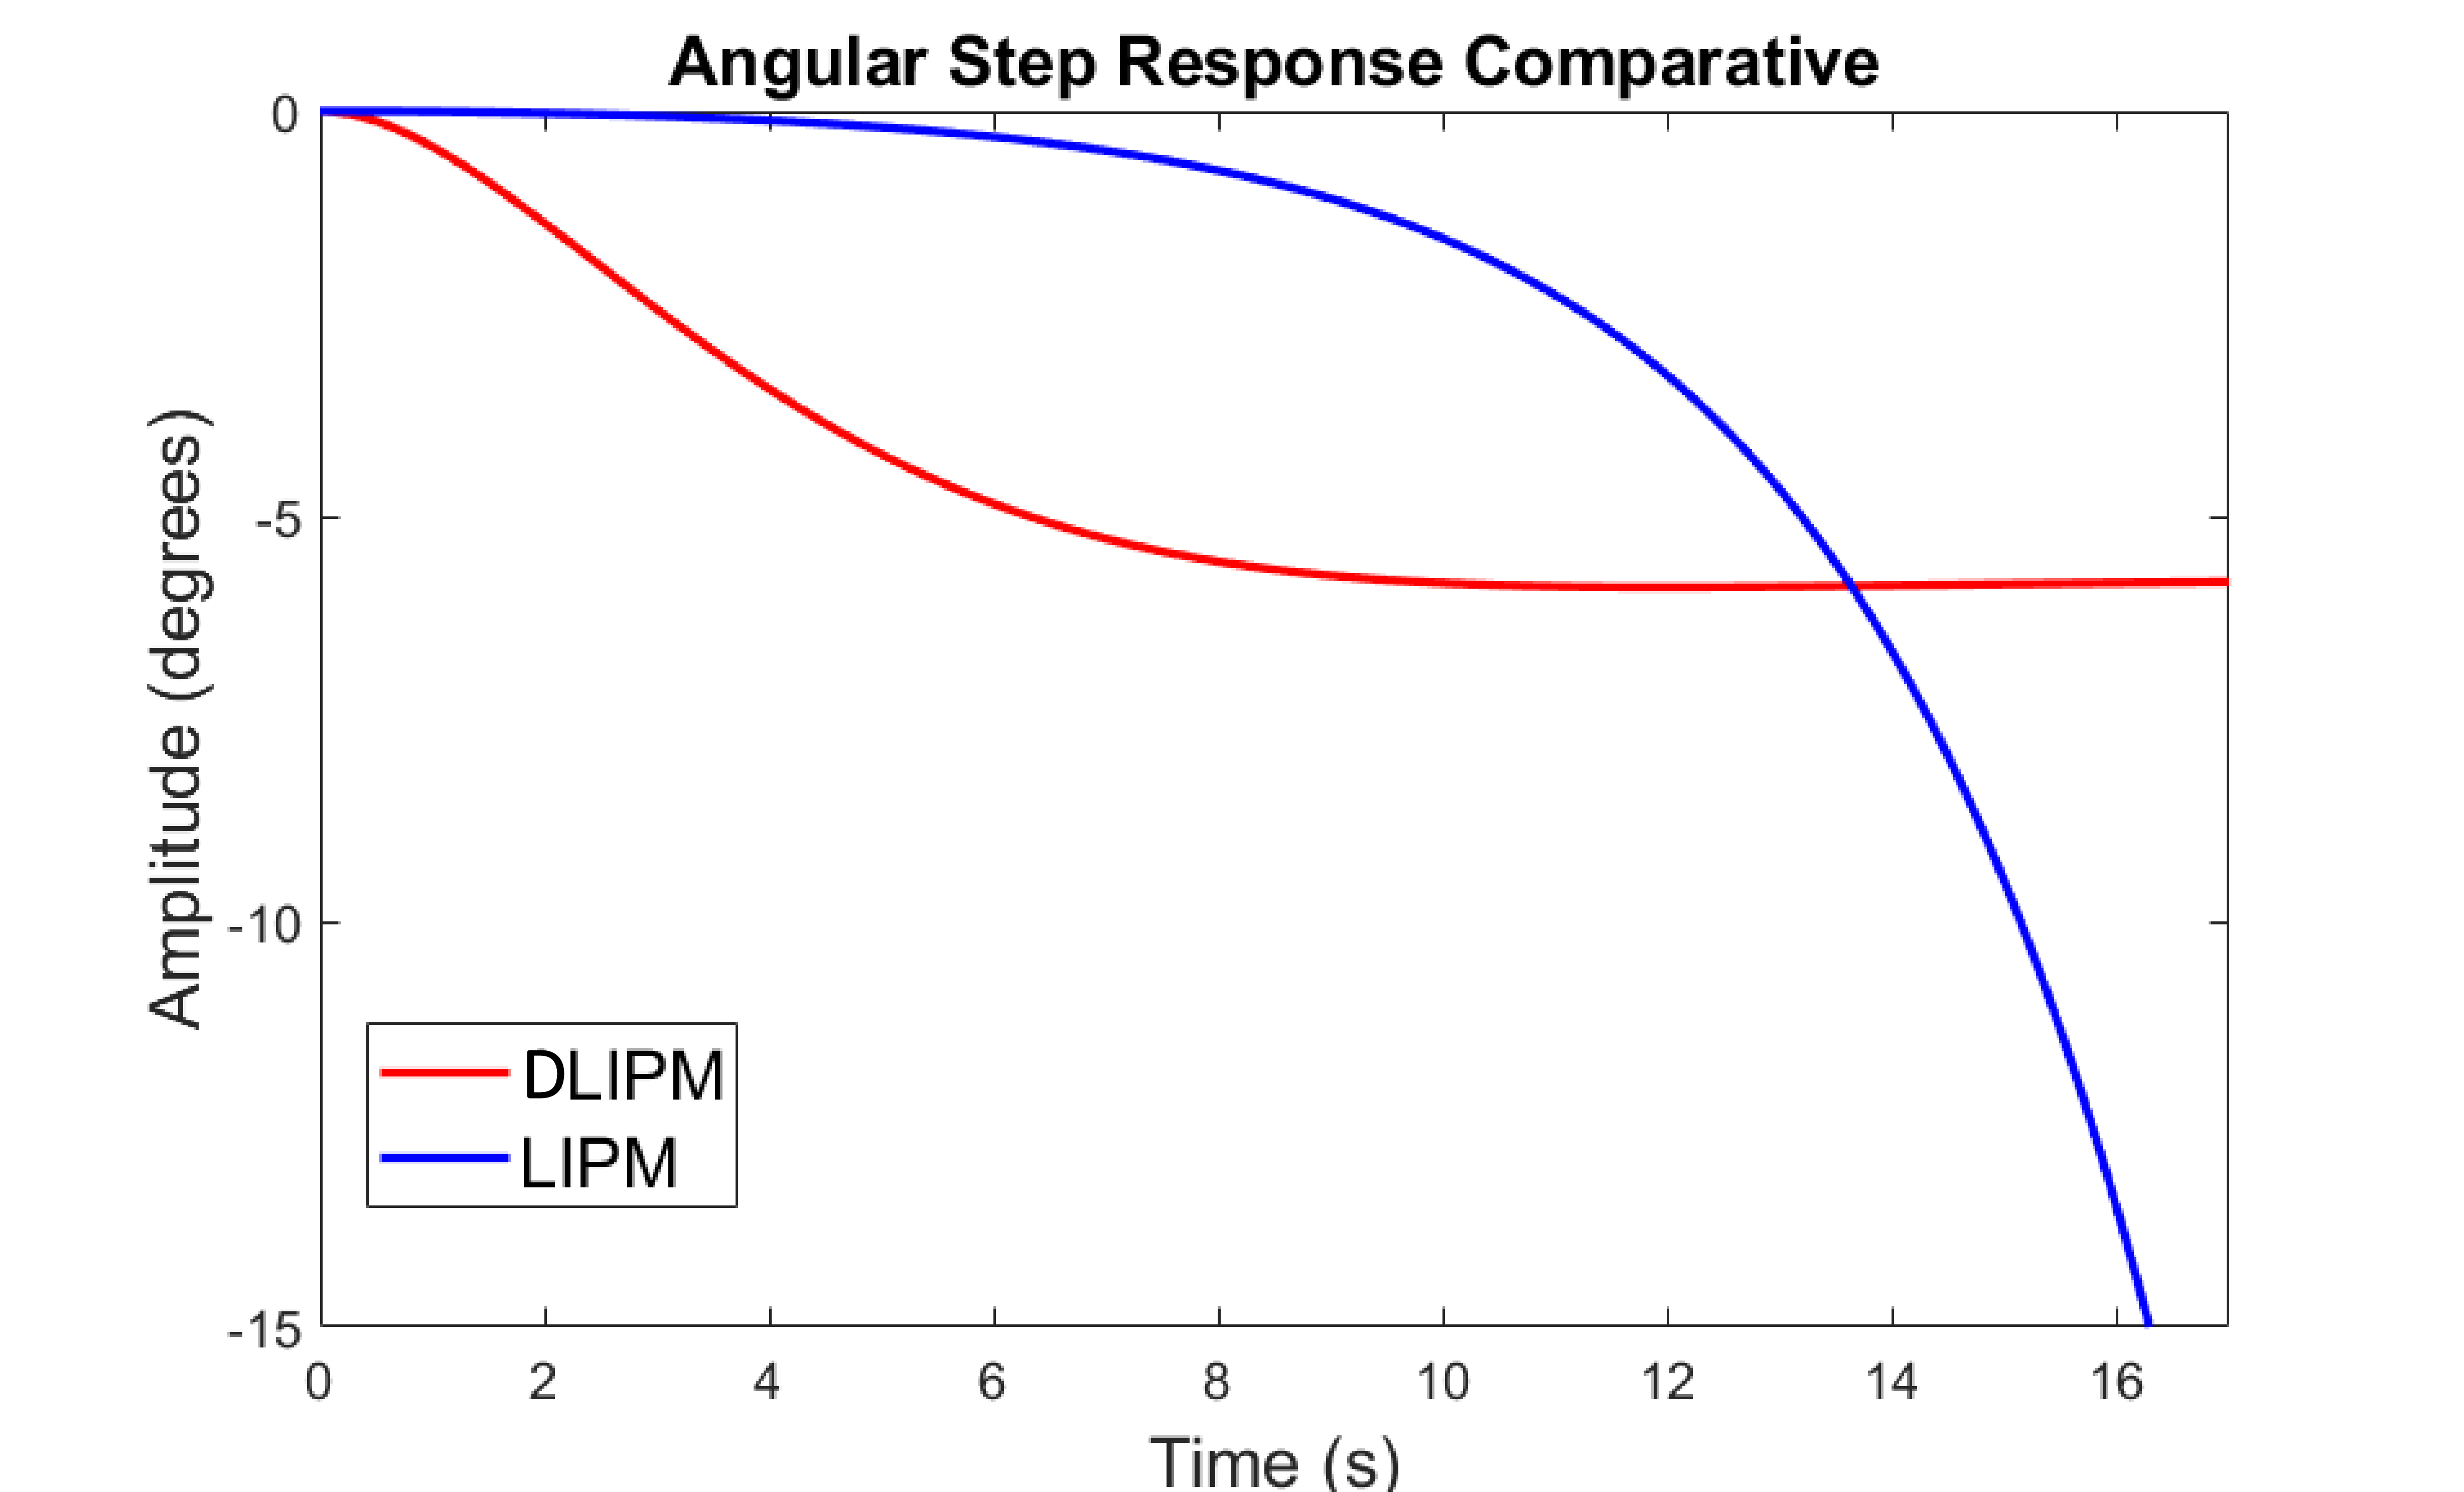
\includegraphics[width=13cm, height=8cm]{imagenes/apartado_5/59_comparativa_paso}
\caption{Comparativa de la respuesta angular entre LIPM y DLIPM}
\label{figura58}
\end{figure}




\textbf{PREGUNTAR A SANTI SI AÑADO LA GRÁFICA 18 DEL PAPER AQUÍ}

\end{itemize}




\subsubsection{Control de ZMP}



\subsubsection{Validación de datos experimental}

Se realizaron diversos experimentos con el nuevo modelo DLIPM, que consistían en la variación del ZMP deseado para visualizar la respuesta del nuevo sistema de control. Se siguió la misma metodología que para el modelo LIPM. Se comandaba un $ZMP_{ref}$ que se transofrmaba en ángulo, para que el robot se inclinara. 



\begin{figure}[H]
\centering
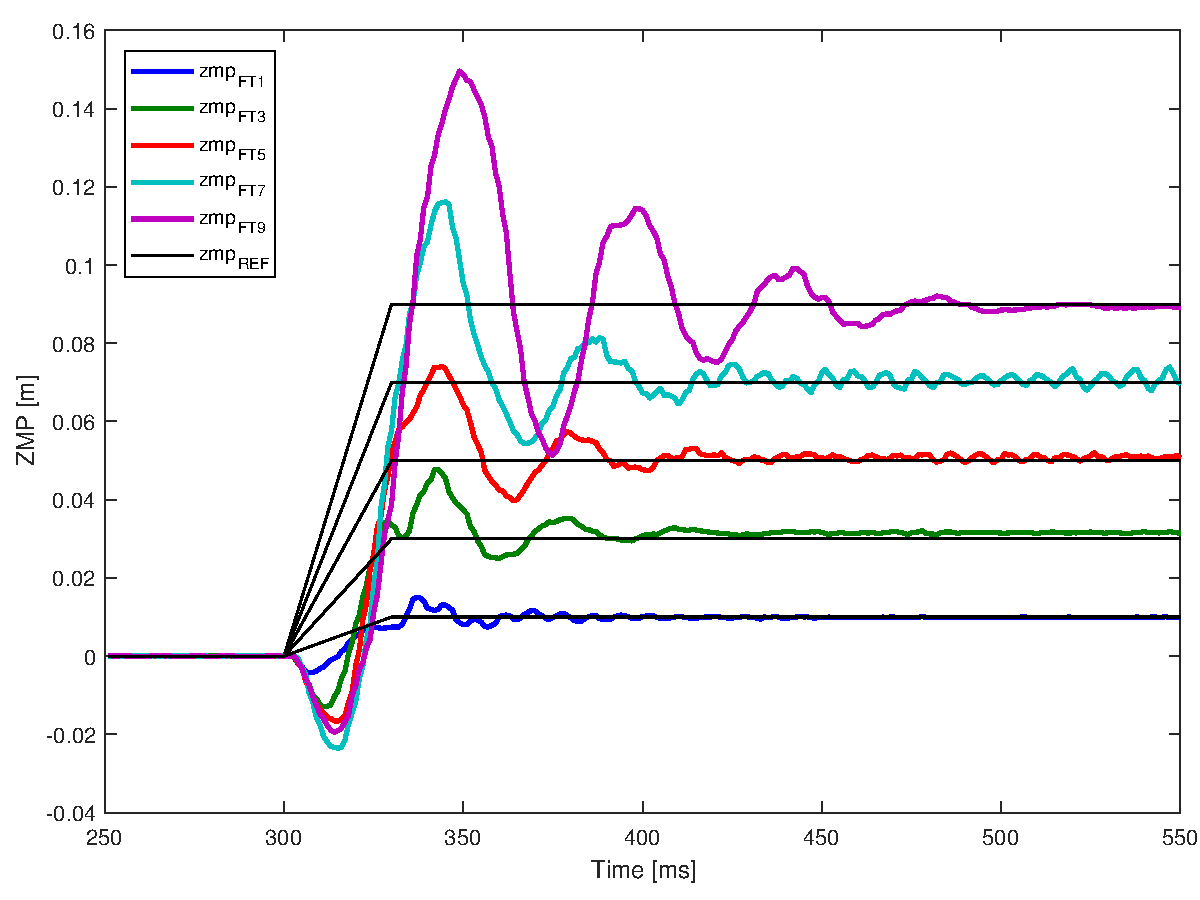
\includegraphics[width=13cm, height=8cm]{imagenes/apartado_5/figura4.pdf}
\caption{Evolucion ZMP modelo DLIPM}
\label{figura55}
\end{figure}

\subsection{Estudio de la respuesta del sensor inercial IMU}\label{respuestaIMU}

\subsubsection{Descripción de la metodología experimental}

Para los experimentos del modelo cart-table, se siguió la misma metodología de inicio del robot que para el modelo LIPM:

\begin{enumerate}
\item \textbf{Puesta del robot en posición inicial (Homeposs)}\\

\item \textbf{Corrección offset sensores F-T} 

\item \textbf{Puesta en marcha del sensor inercial IMU}\\ Una vez que se han realizado los dos pasos anteriores, se debe iniciar la IMU para poder obtener datos de aceleraciones del robot para calcular la altura $z_{CoM}$ del modelo cart-table a partir del ZMP del modelo DLIPM. Por último, se baja el robot antes de iniciar el programa.

\item \textbf{Puesta en marcha del programa}\\ Una vez que se ha puesto en marcha el programa, éste realiza la primera fase igual que en los anteriores experimentos. 
%%\textbf{Corrección offset sensores F-T}\\ Ya realizada la posición de inicio del robot, desde una terminal se deben iniciar los sensores F-T de los tobillos que se van a encargar de dar la información de las fuerzas y los pares al programa para así poder realizar los experimentos, siempre con el robot en suspensión para eliminar los posibles offset que puedan tener los mismos. Es importante que no esté apoyado en el suelo para que cuando se ejecute esta corrección, no se elimine el valor de la fuerza ejercida por la masa del robot. Una vez que se han iniciado los sensores F-T de los tobillos ya se podría bajar el robot para que éstos puedan tener en cuenta el propio peso del robot y las demás fuerzas y pares.
\end{enumerate}




\afterpage{\null\newpage}
\newpage
